\documentclass[aspectratio=169]{beamer}
\usepackage[utf8]{inputenc}
\usepackage[italian]{babel}
\usepackage{amsmath}
\usepackage{graphicx}
\usepackage{tikz}
\usepackage{xcolor}
%
%=====================================================================
%
% Tema e colori
\usetheme{Madrid}
\usecolortheme{seahorse}
%
%=====================================================================
%
% Definizione colori personalizzati
\definecolor{aiblue}{RGB}{30,144,255}
\definecolor{mlgreen}{RGB}{46,139,87}
\definecolor{datacolor}{RGB}{255,140,0}
%
%=====================================================================
%
\begin{document}
%
%=====================================================================
%
\begin{frame}
    \centering
    
\includegraphics[width=\textwidth]{./pics/bibliografia.png}
\end{frame}
%
%..................................................................
%
\begin{frame}
\frametitle{\small M. Ranieri, S. Cuomo, G. Biagini \\ \normalsize \textbf{Scuola e Intelligenza Artificiale}}
\begin{columns}[c]
% Colonna sinistra con l'immagine del libro
\begin{column}{0.35\textwidth}
    \centering
    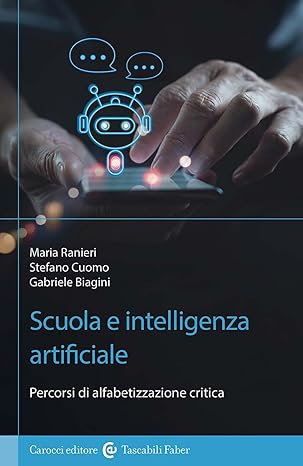
\includegraphics[width=0.75\textwidth]{./pics/ranieri_cover.jpg}
\end{column}
% Colonna destra con la sinossi
\begin{column}{0.6\textwidth}
    {\small
    L'intelligenza artificiale (IA) non è più materia soltanto da esperti di computer science. Le sue applicazioni sono sempre più diffuse e il loro carattere spesso rende difficile comprendere i contorni del binomio naturale-artificiale, con evidenti implicazioni di carattere etico. Le applicazioni di IA, infatti, sono tanto più efficaci quanto più ampia è la base di dati di cui possono avvalersi, dati che sono forniti  dagli utenti stessi dell'ecosistema digitale. Capire la grammatica dell'IA diventa perciò cruciale e la scuola può svolgere un ruolo centrale nella promozione di una literacy critica sui processi di automazione delle nostre società. Il volume offre un quadro di riferimento per lo sviluppo di competenze sull'uso attivo e consapevole dell'IA e propone percorsi di alfabetizzazione critica che gli insegnanti possono realizzare in classe.}
\end{column}
\end{columns}
\end{frame}
%
%..................................................................
%
\begin{frame}
\frametitle{\small L. Di Filippo  \\ \normalsize \textbf{Intelligenza Artificiale per Docenti}}
\begin{columns}[c]
% Colonna sinistra con l'immagine del libro
\begin{column}{0.35\textwidth}
    \centering
    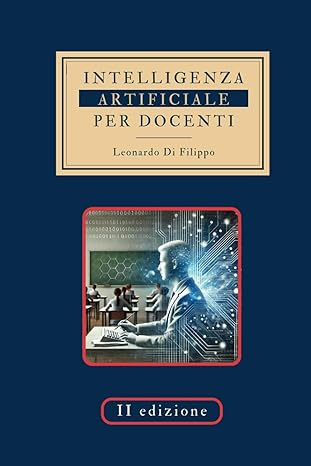
\includegraphics[width=0.75\textwidth]{./pics/difilippo-cover.jpg}
\end{column}
% Colonna destra con la sinossi
\begin{column}{0.6\textwidth}
    {\small
Intelligenza Artificiale per Docenti è un'opera concepita per guidare gli insegnanti nell’esplorazione e nell’uso pratico dell’intelligenza artificiale (AI) in ambito scolastico.
Il libro offre una panoramica sulle tecnologie AI e, attraverso esempi concreti, una rassegna dei possibili campi applicativi. La struttura del testo è agile e orientata all’essenziale, ma include non pochi contenuti di approfondimento online, consultabili facilmente tramite codici QR durante la lettura. Non mancano riflessioni sull’utilizzo dell’intelligenza artificiale, con particolare attenzione alla supervisione umana e alle implicazioni sociali ed etiche.}
\end{column}
\end{columns}
\end{frame}
%
%..................................................................
%
\begin{frame}
\frametitle{\small L. Floridi \\ \normalsize \textbf{Etica dell'intelligenza artificiale. Sviluppi, opportunità, sfide}}
\begin{columns}[c]
% Colonna sinistra con l'immagine del libro
\begin{column}{0.35\textwidth}
    \centering
    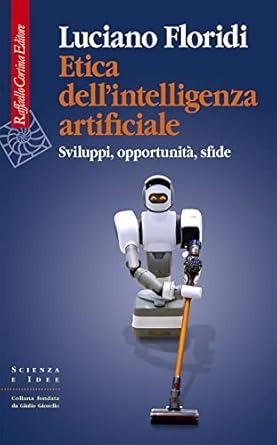
\includegraphics[width=0.75\textwidth]{./pics/floridi_cover.jpg}
\end{column}
% Colonna destra con la sinossi
\begin{column}{0.6\textwidth}
    {\small
    Istruzione, commercio, industria, viaggi, divertimento, sanità, politica, relazioni sociali, in breve la vita stessa sta diventando inconcepibile senza le tecnologie, i servizi, i prodotti digitali. Questa trasformazione epocale implica dubbi e preoccupazioni, ma anche straordinarie opportunità. Proprio perché la rivoluzione digitale è iniziata da poco abbiamo la possibilità di modellarla in senso positivo, a vantaggio dell’umanità e del pianeta. Ma a condizione di capire meglio di cosa stiamo parlando. È cruciale comprendere le trasformazioni tecnologiche in atto e uno dei passaggi oggi fondamentali è quello dell’intelligenza artificiale, della sua natura e delle sue sfide etiche, che Luciano Floridi affronta in questo libro, offrendo il suo contributo di idee a un quanto mai necessario sforzo collettivo di intelligenza.}
\end{column}
\end{columns}
\end{frame}
%
%..................................................................
%
\begin{frame}
\frametitle{\small A. Ananthaswamy \\ \normalsize \textbf{Perché le Macchine Imparano: L'Eleganza della Matematica dietro l'AI}}
\begin{columns}[c]
% Colonna sinistra con l'immagine del libro
\begin{column}{0.35\textwidth}
    \centering
    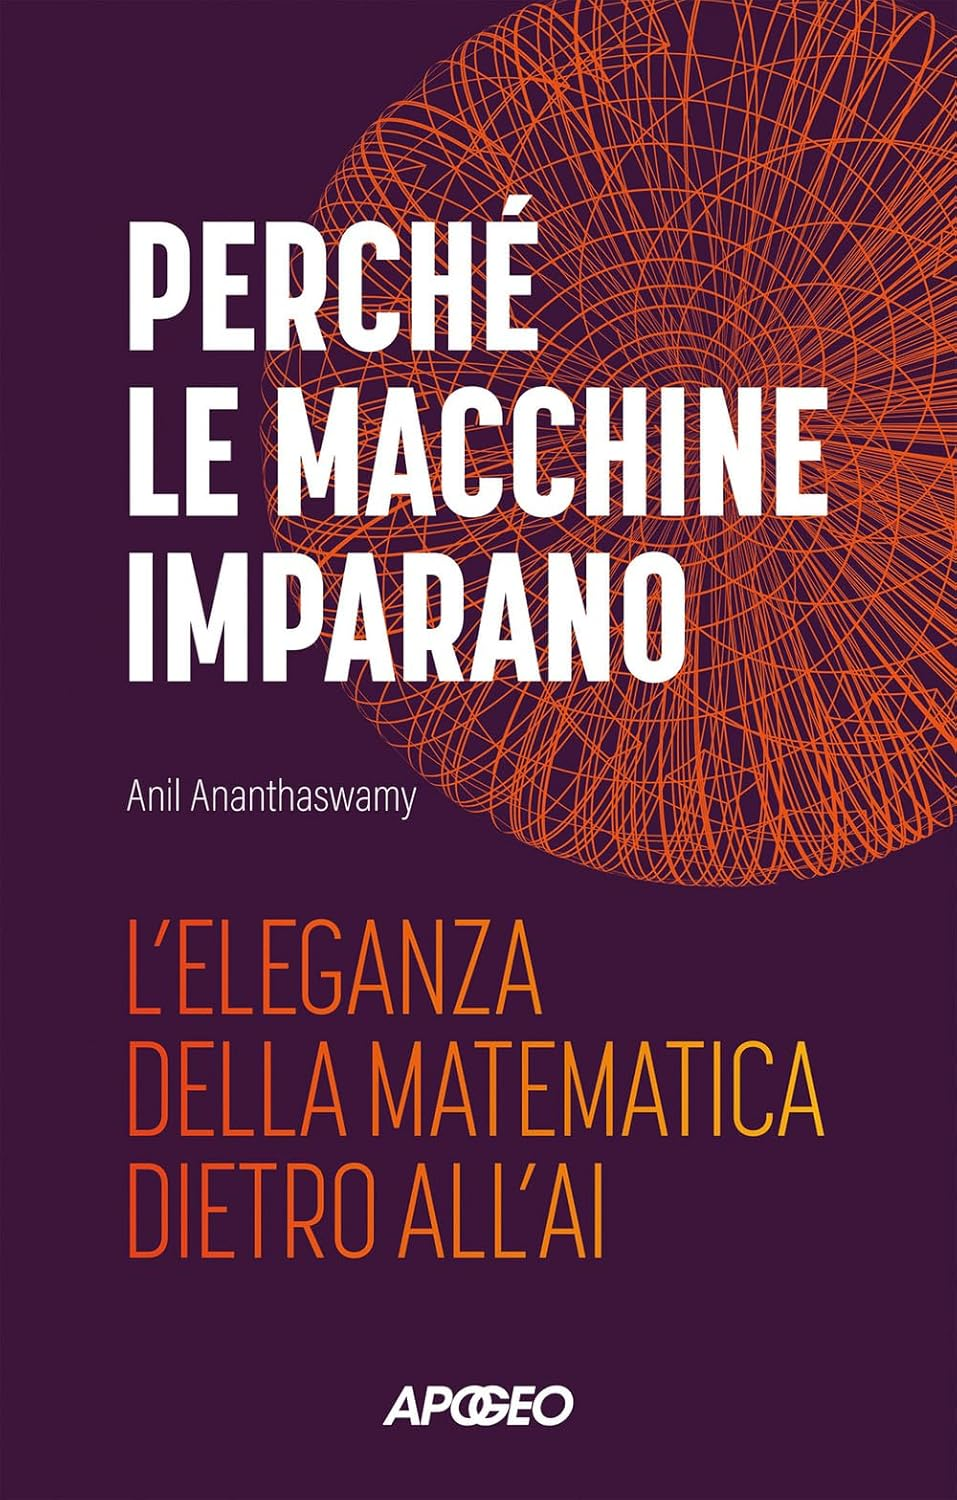
\includegraphics[width=0.75\textwidth]{./pics/ananth_cover.jpg}
\end{column}
% Colonna destra con la sinossi
\begin{column}{0.6\textwidth}
    {\small
    Le macchine prendono da tempo decisioni che impattano sulle nostre vite: approvano prestiti ipotecari, determinano se un tumore è maligno, influenzano gli sviluppi e le scoperte in chimica, biologia e fisica. Negli ultimi tempi, con l'entrata in scena delle cosiddette AI generative come ChatGPT, la loro importanza è cresciuta ancora. Dietro alle macchine intelligenti ci sono idee matematiche relativamente semplici, alcune delle quali risalgono a secoli fa, per esempio l'algebra lineare e il calcolo. In questo libro illuminante, Anil Ananthaswamy spiega la matematica che permette alla macchine di imparare, suggerendo al contempo intriganti collegamenti tra intelligenza artificiale e umana: e se la matematica fosse la chiave di lettura per entrambe?}
\end{column}
\end{columns}
\end{frame}
%
%..................................................................
%
\begin{frame}
\frametitle{\small V. Mellano \\ \normalsize \textbf{E Tu l'Hai Capita l'AI? L'Intelligenza Artificiale in Poche Parole}}
\begin{columns}[c]
% Colonna sinistra con l'immagine del libro
\begin{column}{0.35\textwidth}
    \centering
    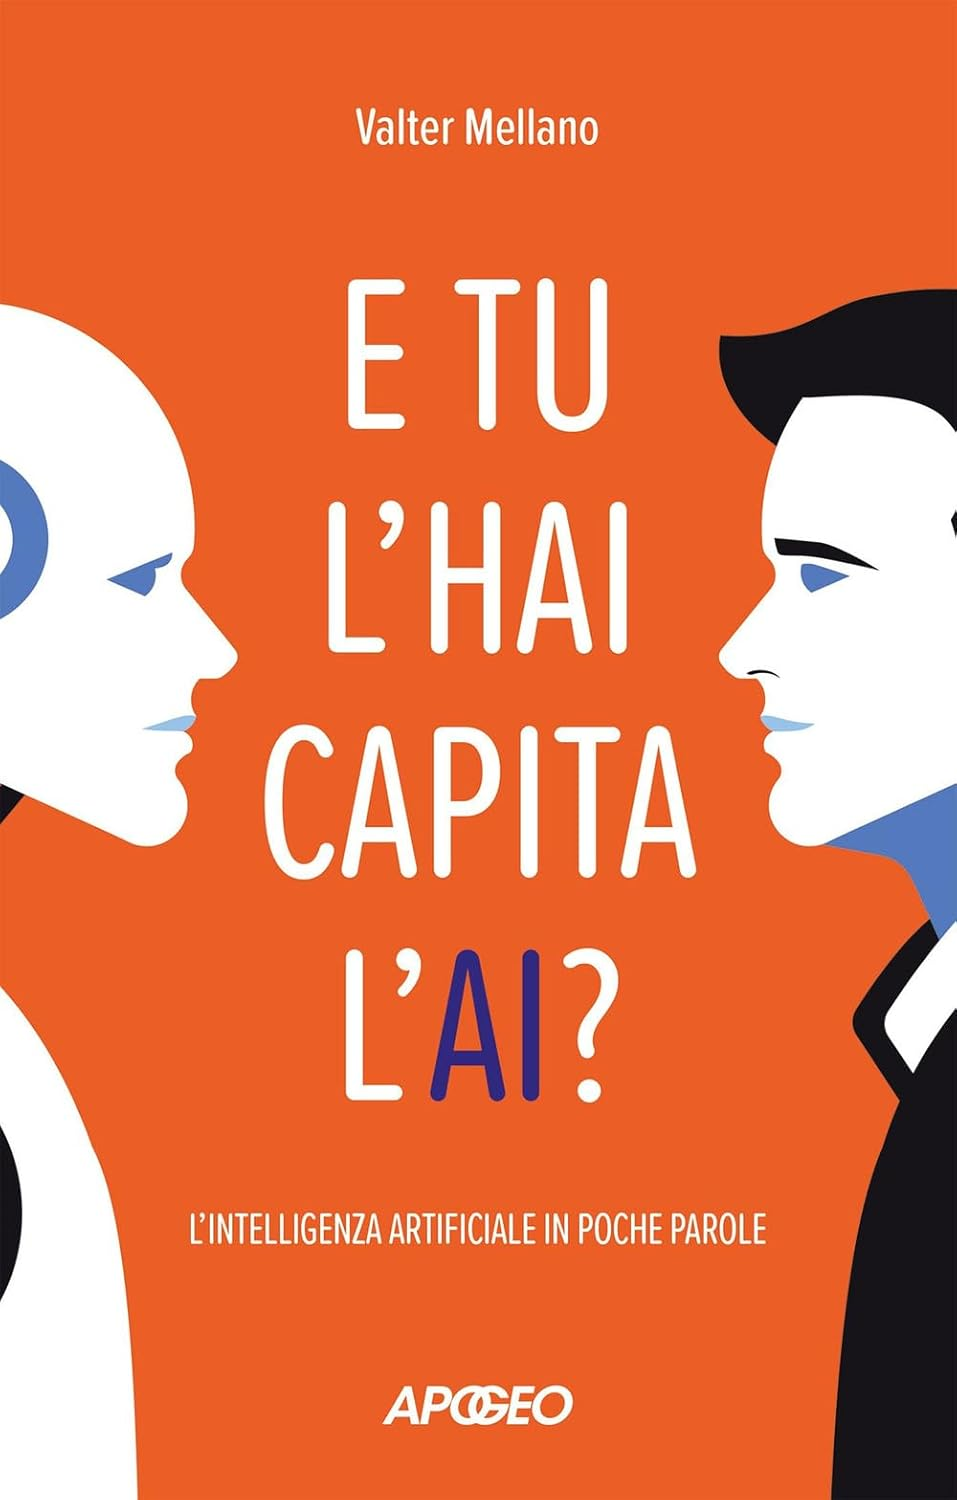
\includegraphics[width=0.75\textwidth]{./pics/mellano_cover.jpg}
\end{column}
% Colonna destra con la sinossi
\begin{column}{0.6\textwidth}
    {\small
    "E tu l’hai capita l’AI?" smonta e analizza la tecnologia dietro l’intelligenza artificiale in modo semplice e comprensibile anche a chi ha solo una conoscenza basilare della matematica e nessuna di programmazione. Dopo aver mostrato che cosa è e come funziona, l’autore affronta i temi più attuali, come i cambiamenti nel mondo del lavoro e l’impatto sulla società, presentando un'analisi dei rischi e delle opportunità, senza trascurare gli aspetti etici, legali e quelli più insoliti come le allucinazioni dell’AI generativa. L’obiettivo è presentare l'intelligenza artificiale a chi ha la curiosità di vedere "cosa c'è dentro", fornendo una visione completa senza dare nulla per scontato.}
\end{column}
\end{columns}
\end{frame}
%
%..................................................................
%
\begin{frame}
\frametitle{\small E. Bezzecchi \\ \normalsize \textbf{Intelligenza Artificiale}}
\begin{columns}[c]
% Colonna sinistra con l'immagine del libro
\begin{column}{0.35\textwidth}
    \centering
    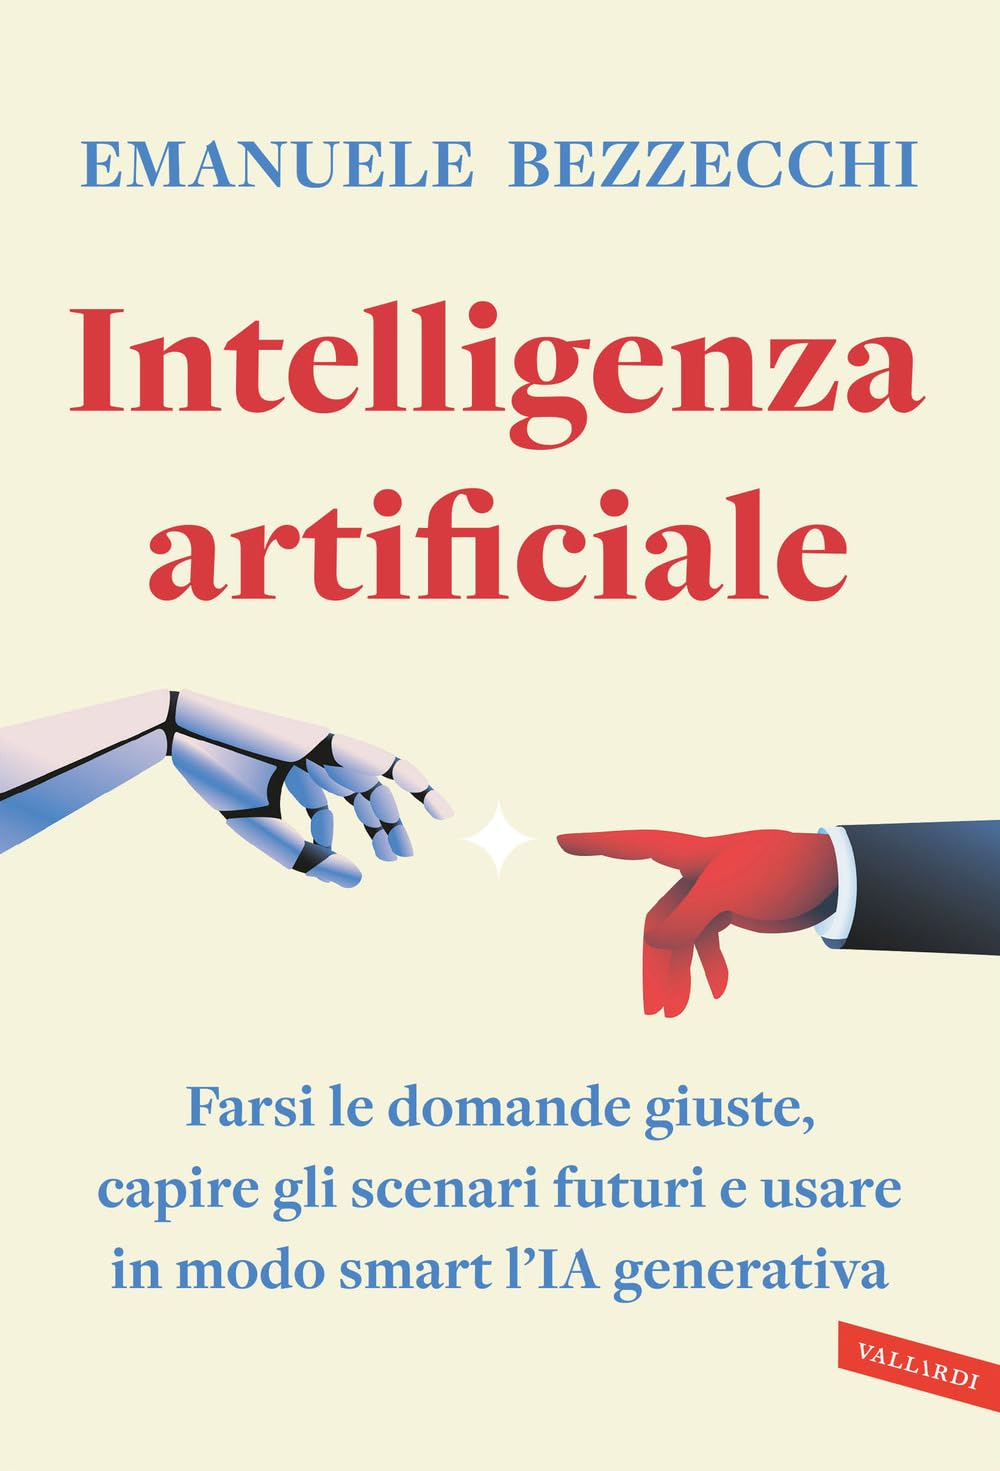
\includegraphics[width=0.75\textwidth]{./pics/bezzecchi_cover.jpg}
\end{column}
% Colonna destra con la sinossi
\begin{column}{0.6\textwidth}
    {\small
    Intelligenza artificiale: ispira meraviglia, incute timore… Ma cosa dobbiamo aspettarci? Da sempre le macchine sono più efficienti degli umani nel fare calcoli, mentre ciò che distingue l’umano è la sua capacità di pensare in maniera originale e utilizzare le parole per esprimere le proprie idee. Almeno finora. Adesso che questa distinzione si sta facendo più sottile, è necessario capire che cos’è e di che cosa è capace l’IA generativa. Emanuele Bezzecchi, esperto di IA e Open Innovation, ci guida con un linguaggio chiaro e accessibile nel capire come è nata e come usarla, quali sono i suoi meccanismi interni e i suoi limiti. Un libro pratico che è la risposta ai tanti quesiti che ci pone oggi la tecnologia, uno strumento agile e aggiornato per capire e affrontare le sfide che il futuro ci riserva.}
\end{column}
\end{columns}
\end{frame}
%
%..................................................................
%
\begin{frame}
\frametitle{\small G. Vessio \\ \normalsize \textbf{Intelligenza Artificiale per Curiosi}}
\begin{columns}[c]
% Colonna sinistra con l'immagine del libro
\begin{column}{0.35\textwidth}
    \centering
    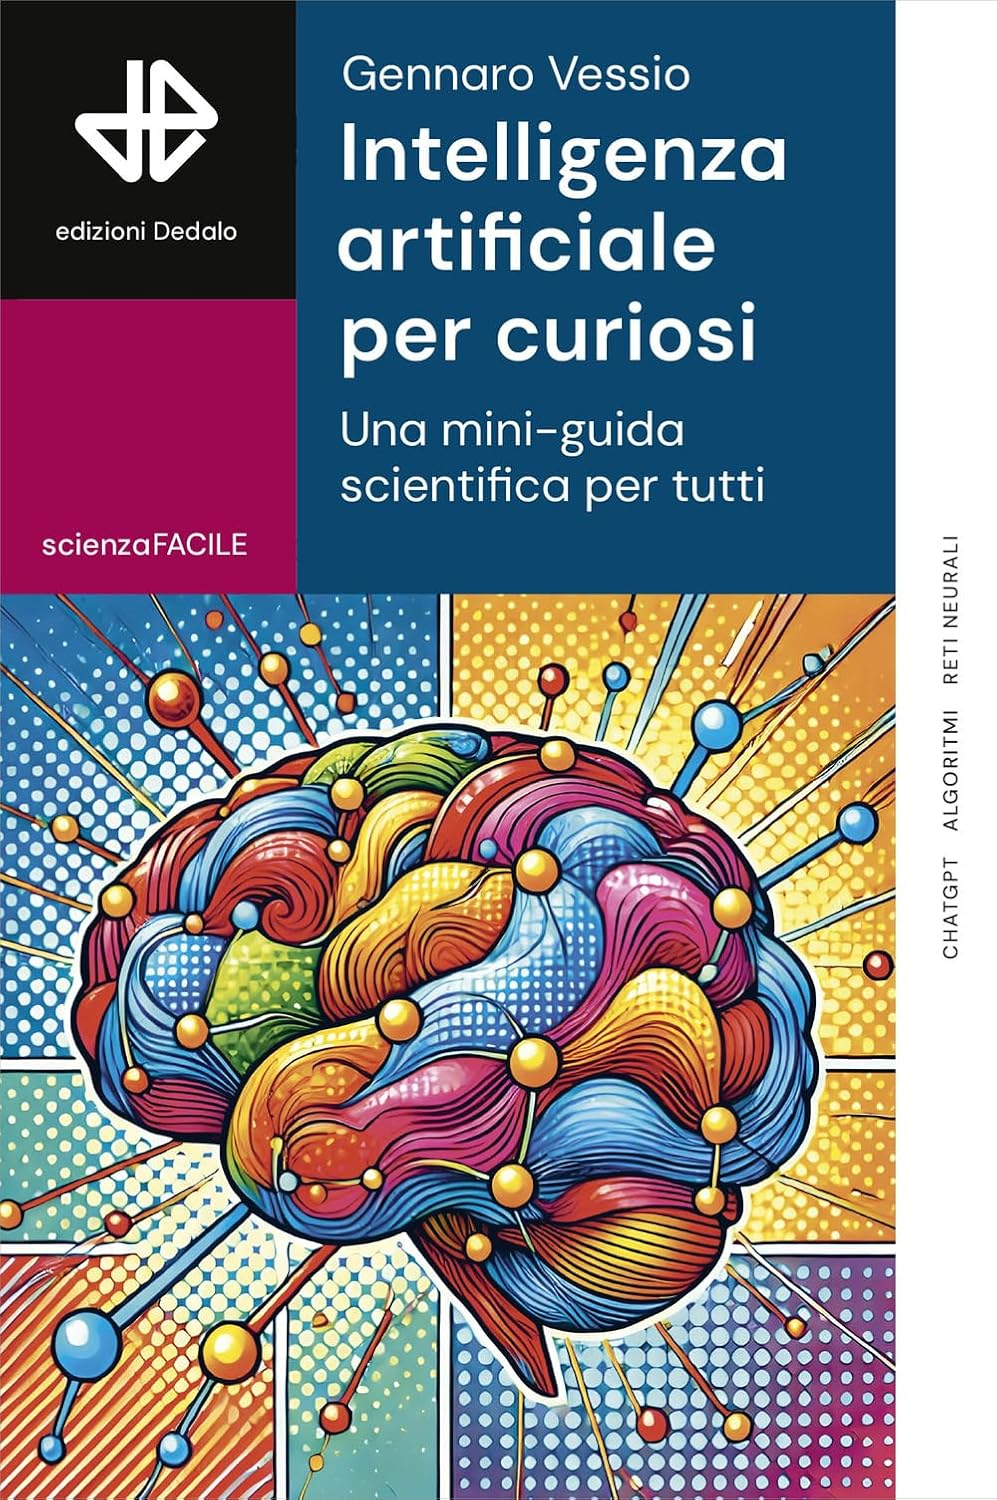
\includegraphics[width=0.75\textwidth]{./pics/vessio_cover.jpg}
\end{column}
% Colonna destra con la sinossi
\begin{column}{0.6\textwidth}
    {\small
    In questa guida accessibile e didattica insieme, l’autore esplora i concetti chiave dell’intelligenza artificiale, ripercorrendone l'evoluzione storica e analizzando le tecnologie alla base di questa rivoluzione: dalle reti neurali artificiali ai chatbot e agli assistenti digitali che stanno trasformando le nostre vite. L’obiettivo è demistificare l’argomento e chiarire i meccanismi che consentono alle macchine di “simulare” un comportamento intelligente. Attraverso metafore intuitive ed esempi calati nel quotidiano, il libro è una lettura ideale per chi è curioso di dare un’occhiata a cosa si cela “dietro le quinte” delle tecnologie che stanno cambiando il mondo.}
\end{column}
\end{columns}
\end{frame}
%
%..................................................................
%
\begin{frame}
\frametitle{\small B. Di Bello \\ \normalsize \textbf{IA Generativa for Dummies}}
\begin{columns}[c]
% Colonna sinistra con l'immagine del libro
\begin{column}{0.35\textwidth}
    \centering
    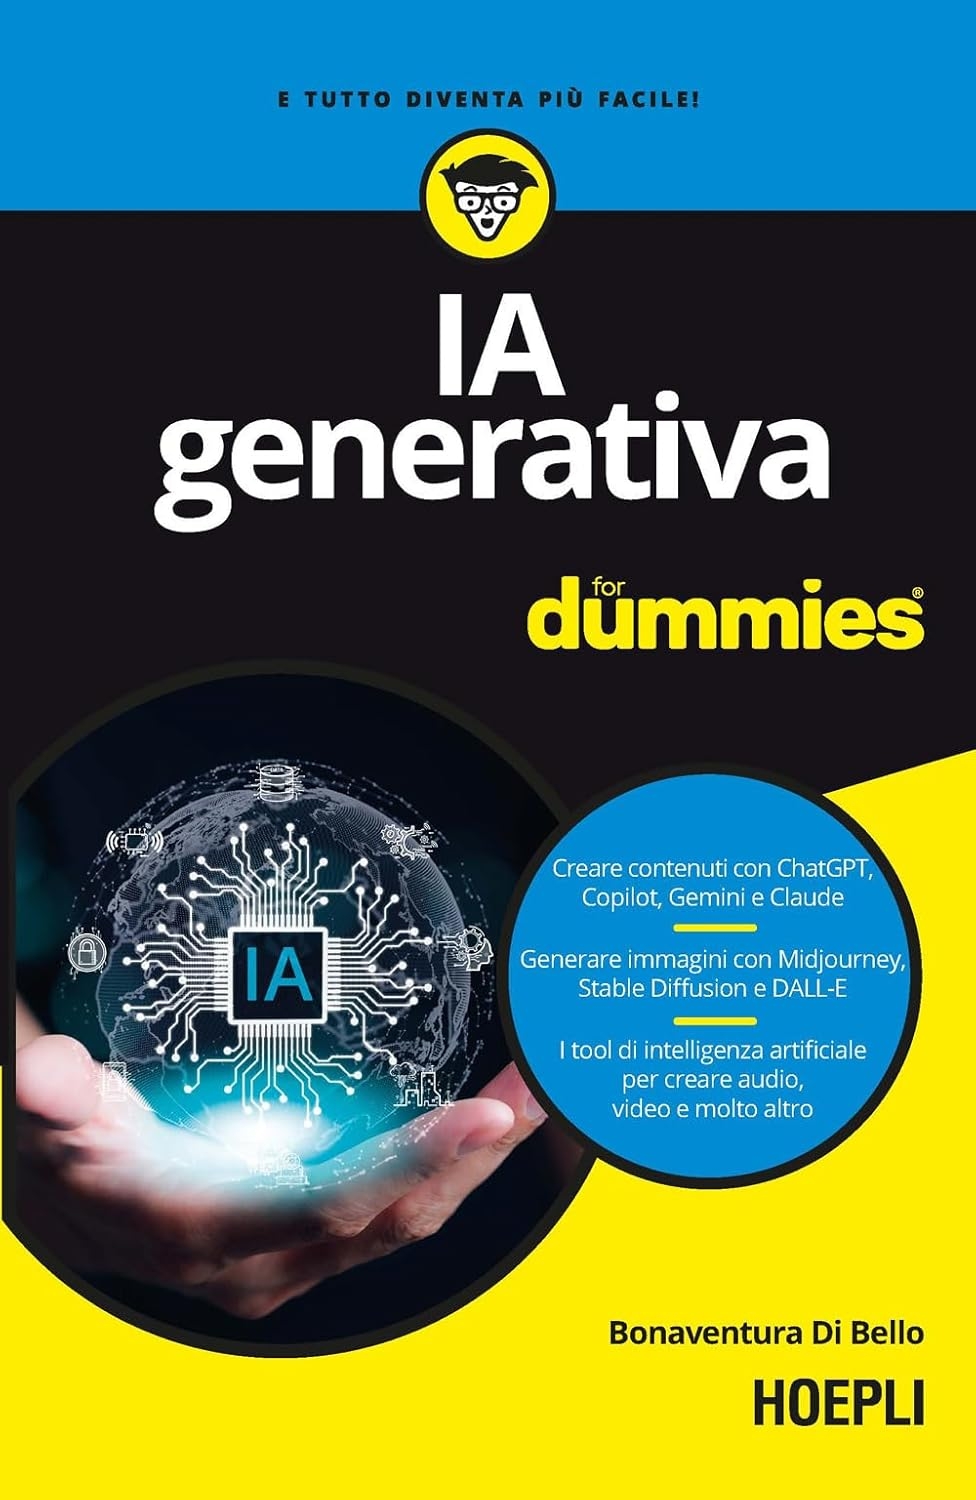
\includegraphics[width=0.75\textwidth]{./pics/dibello_cover.jpg}
\end{column}
% Colonna destra con la sinossi
\begin{column}{0.6\textwidth}
    {\small
I nuovi modelli di Intelligenza Artificiale generativa per il testo e per le immagini offrono infinite opportunità a chi sa come interrogarli, trasformandoli in preziosi assistenti digitali in qualsiasi campo. Con questa nuova guida avrete a disposizione tutte le idee e le strategie più efficaci per ottenere i risultati che desiderate, tanto in ambito personale quanto professionale, ponendo al vostro chatbot preferito le domande giuste in ogni occasione. Con un approccio graduale e ricco di esempi pratici, esplorerete tutte le diverse possibilità di generazione ed elaborazione di contenuti di testo e immagini. Una serie di prompt efficaci pronti per l’uso vi guideranno nell’interrogazione, garantendo i risultati migliori in ogni occasione.
}
\end{column}
\end{columns}
\end{frame}
%
%..................................................................
%
\begin{frame}
\frametitle{\small G. Roncaglia  \\ \normalsize \textbf{L'Architetto e l'Oracolo}}
\begin{columns}[c]
% Colonna sinistra con l'immagine del libro
\begin{column}{0.35\textwidth}
    \centering
    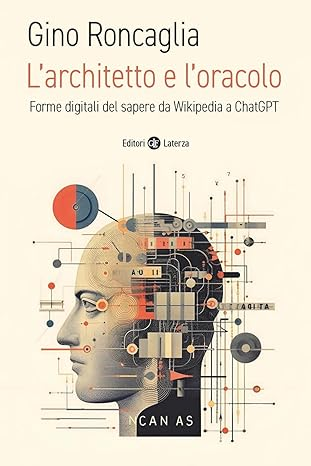
\includegraphics[width=0.75\textwidth]{./pics/roncaglia_cover.jpg}
\end{column}
% Colonna destra con la sinossi
\begin{column}{0.6\textwidth}
    {\small
Per comprendere il significato e la portata di della rivoluzione dell'AI, bisogna collocarla nel contesto di quello che è stato, da millenni, un sogno dell’umanità: organizzare il sapere in modo da poterlo trasmettere, recuperare, utilizzare, accrescere nelle forme di volta in volta più funzionali rispetto ai nostri molteplici e diversi obiettivi. E bisogna capire le idee e i principi che sono alla base degli strumenti non solo tecnologici ma anche sociali e culturali che stiamo creando all’interno del nuovo ecosistema digitale.
}
\end{column}
\end{columns}
\end{frame}
%
%..................................................................
%
\begin{frame}
\frametitle{\small N. Cristianini   \\ \normalsize \textbf{La Scorciatoia}}
\begin{columns}[c]
% Colonna sinistra con l'immagine del libro
\begin{column}{0.35\textwidth}
    \centering
    
\includegraphics[width=0.75\textwidth]{./pics/cristianini-1-cover.jpg}
\end{column}
% Colonna destra con la sinossi
\begin{column}{0.6\textwidth}
    {\small
Vagliano curricula, concedono mutui, scelgono le notizie che leggiamo: le macchine intelligenti sono entrate nelle nostre vite. Fanno molte delle cose che volevamo, e anche qualcuna in più, ma non possiamo capirle o ragionare con loro, perché il loro comportamento è in realtà guidato da relazioni statistiche ricavate da quantità sovrumane di dati.  E allora come incorporarle nella nostra società senza rischi ed effetti collaterali? Questo libro ci spiega come siamo arrivati sin qui, e indica il percorso che ci aspetta prima di poterci fidare di questi nuovi agenti «alieni». La tecnologia non basta, occorre un dialogo tra scienze naturali e umane: è il passaggio cruciale per una convivenza sicura con questa nuova forma di intelligenza.
}
\end{column}
\end{columns}
\end{frame}
%
%..................................................................
%
\begin{frame}
\frametitle{\small N. Cristianini   \\ \normalsize \textbf{Machina Sapiens}}
\begin{columns}[c]
% Colonna sinistra con l'immagine del libro
\begin{column}{0.35\textwidth}
    \centering
    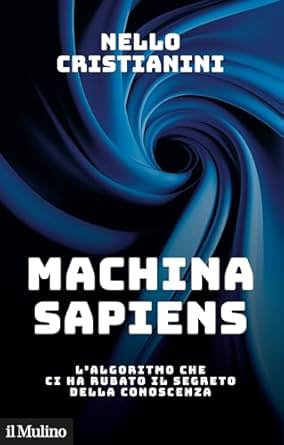
\includegraphics[width=0.75\textwidth]{./pics/cristianini-2-cover.jpg}
\end{column}
% Colonna destra con la sinossi
\begin{column}{0.6\textwidth}
    {\small
Le macchine possono pensare? Questa domanda inquietante, posta da Alan Turing nel 1950, ha forse trovato una risposta: oggi si può conversare con un computer senza poterlo distinguere da un essere umano. I nuovi agenti intelligenti come ChatGPT si sono rivelati capaci di svolgere compiti che vanno molto oltre le intenzioni iniziali dei loro creatori, e ancora non sappiamo perché: se sono stati addestrati per alcune abilità, altre sono emerse spontaneamente mentre leggevano migliaia di libri e milioni di pagine web.
È questo il segreto della conoscenza, ed è adesso nelle mani delle nostre creature? Cos'altro può emergere, mentre continuiamo su questa strada?
}
\end{column}
\end{columns}
\end{frame}
%
%..................................................................
%
\begin{frame}
\frametitle{\small N. Cristianini   \\ \normalsize \textbf{Sovrumano}}
\begin{columns}[c]
% Colonna sinistra con l'immagine del libro
\begin{column}{0.35\textwidth}
    \centering
    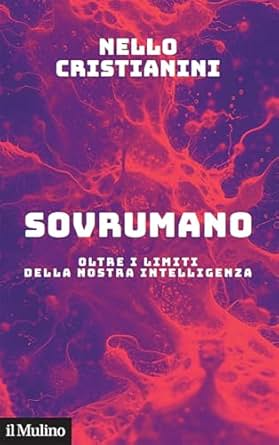
\includegraphics[width=0.75\textwidth]{./pics/cristianini-3-cover.jpg}
\end{column}
% Colonna destra con la sinossi
\begin{column}{0.6\textwidth}
    {\small
La domanda oggi è cambiata: non è più se le macchine possono essere intelligenti, ma se possono eguagliarci e superarci. L'intelligenza artificiale sta ormai raggiungendo le prestazioni umane  su molti dei compiti cognitivi in cui eccelliamo. Ma cosa avverrà dopo? Stiamo entrando in un'epoca in cui le macchine saranno in grado di capire cose per noi incomprensibili? Nessuna intelligenza è illimitata, nemmeno la nostra, e quindi ci chiediamo: cosa si trova al di là dei limiti umani? Ma mentre investiamo grandi capitali per costruire una macchina in grado di competere con noi, ci rifiutiamo di accettare che questo sia possibile. Desideriamo e al tempo stesso temiamo quell'incontro. 
}
\end{column}
\end{columns}
\end{frame}
%
%..................................................................
%
\begin{frame}
\frametitle{\small L. Perilli  \\ \normalsize \textbf{Coscienza Artificiale}}
\begin{columns}[c]
% Colonna sinistra con l'immagine del libro
\begin{column}{0.35\textwidth}
    \centering
    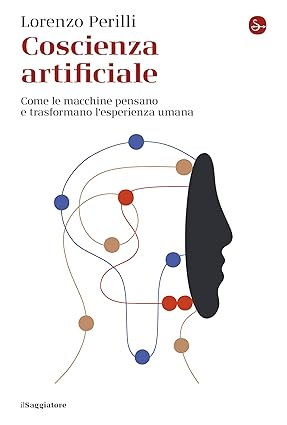
\includegraphics[width=0.75\textwidth]{./pics/perilli-cover.jpg}
\end{column}
% Colonna destra con la sinossi
\begin{column}{0.6\textwidth}
    {\small
A partire dalle riflessioni di Omero e Aristotele, Cartesio e Leibniz, Norbert Wiener e Douglas Hofstadter, Coscienza artificiale ci spinge a riflettere su tematiche che mai gli esseri umani si sono trovati ad affrontare prima che l'evoluzione delle macchine li costringesse a farlo. Un'opera profonda e innovativa, che ci rivela come la tecnologia di oggi non sia più stolida materia inerte o qualcosa che reagisce alle nostre sollecitazioni, ma un vero e proprio soggetto autonomo; e che ciò di fronte a cui potremmo infine trovarci è una nuova forma di esistenza.
}
\end{column}
\end{columns}
\end{frame}
%
%..................................................................
%
\begin{frame}
\frametitle{\small A. Colamedici - S. Arcagni  \\ \normalsize \textbf{L'Algoritmo di Babele}}
\begin{columns}[c]
% Colonna sinistra con l'immagine del libro
\begin{column}{0.35\textwidth}
    \centering
    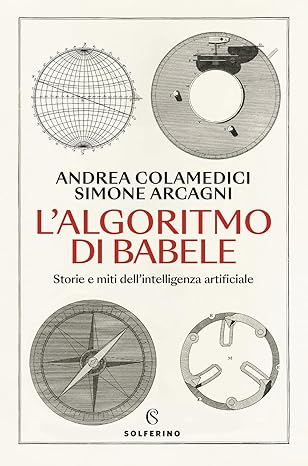
\includegraphics[width=0.75\textwidth]{./pics/colamedici-cover.jpg}
\end{column}
% Colonna destra con la sinossi
\begin{column}{0.6\textwidth}
    {\small
Che cosa ha a che fare Omero con l’intelligenza artificiale? E I viaggi di Gulliver, i trattati di Giordano Bruno, le opere di Borges: cosa ci possono insegnare dell’accelerazione tecnologica?  È proprio esplorando esempi letterari e filosofici come questo che Andrea Colamedici e Simone Arcagni si interrogano sul nostro futuro in relazione all’incredibile sviluppo dell’intelligenza artificiale e al mistero dell’algoritmo di Babele. Attraverso molti capolavori e autori del passato – dai dialoghi di Platone ad Asimov – possiamo infatti ricostruire il codice genetico della nuova frontiera informatica, mostrando come il suo immaginario sia profondamente intrecciato con la nostra società. 
}
\end{column}
\end{columns}
\end{frame}
%
%..................................................................
%
\begin{frame}
\frametitle{\small T. Duke - P. Giudici  \\ \normalsize \textbf{Responsible AI in Practice}}
\begin{columns}[c]
% Colonna sinistra con l'immagine del libro
\begin{column}{0.35\textwidth}
    \centering
    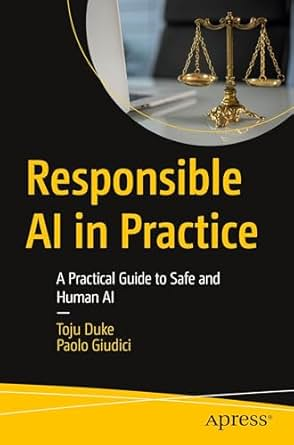
\includegraphics[width=0.75\textwidth]{./pics/giudici-cover.jpg}
\end{column}
% Colonna destra con la sinossi
\begin{column}{0.6\textwidth}
    {\small
This book is the first practical book on AI risk assessment and management. It will enable you to evaluate and implement safe and accurate AI models and applications. The book features risk assessment frameworks, statistical metrics and code, a risk taxonomy curated from real-world case studies, and insights into AI regulation and policy, and is an essential tool for AI governance teams, AI auditors, AI ethicists, machine learning (ML) practitioners, Responsible AI practitioners, and computer science and data science students building safe and trustworthy AI systems across businesses, organizations, and universities.
}
\end{column}
\end{columns}
\end{frame}
%
%=====================================================================
%
\end{document}
%
%=====================================================================
%
%
%..................................................................
%
\begin{frame}
\frametitle{\small   \\ \normalsize \textbf{}}
\begin{columns}[c]
% Colonna sinistra con l'immagine del libro
\begin{column}{0.35\textwidth}
    \centering
    \includegraphics[width=0.75\textwidth]{./pics/_cover.jpg}
\end{column}
% Colonna destra con la sinossi
\begin{column}{0.6\textwidth}
    {\small

}
\end{column}
\end{columns}
\end{frame}
